% Options for packages loaded elsewhere
\PassOptionsToPackage{unicode}{hyperref}
\PassOptionsToPackage{hyphens}{url}
\documentclass[
  10pt,
  a4paper,
]{article}
\usepackage{xcolor}
\usepackage[margin=22mm]{geometry}
\usepackage{amsmath,amssymb}
\setcounter{secnumdepth}{-\maxdimen} % remove section numbering
\usepackage{iftex}
\ifPDFTeX
  \usepackage[T1]{fontenc}
  \usepackage[utf8]{inputenc}
  \usepackage{textcomp} % provide euro and other symbols
\else % if luatex or xetex
  \usepackage{unicode-math} % this also loads fontspec
  \defaultfontfeatures{Scale=MatchLowercase}
  \defaultfontfeatures[\rmfamily]{Ligatures=TeX,Scale=1}
\fi
\usepackage{lmodern}
\ifPDFTeX\else
  % xetex/luatex font selection
\fi
% Use upquote if available, for straight quotes in verbatim environments
\IfFileExists{upquote.sty}{\usepackage{upquote}}{}
\IfFileExists{microtype.sty}{% use microtype if available
  \usepackage[]{microtype}
  \UseMicrotypeSet[protrusion]{basicmath} % disable protrusion for tt fonts
}{}
\makeatletter
\@ifundefined{KOMAClassName}{% if non-KOMA class
  \IfFileExists{parskip.sty}{%
    \usepackage{parskip}
  }{% else
    \setlength{\parindent}{0pt}
    \setlength{\parskip}{6pt plus 2pt minus 1pt}}
}{% if KOMA class
  \KOMAoptions{parskip=half}}
\makeatother
\usepackage{graphicx}
\makeatletter
\newsavebox\pandoc@box
\newcommand*\pandocbounded[1]{% scales image to fit in text height/width
  \sbox\pandoc@box{#1}%
  \Gscale@div\@tempa{\textheight}{\dimexpr\ht\pandoc@box+\dp\pandoc@box\relax}%
  \Gscale@div\@tempb{\linewidth}{\wd\pandoc@box}%
  \ifdim\@tempb\p@<\@tempa\p@\let\@tempa\@tempb\fi% select the smaller of both
  \ifdim\@tempa\p@<\p@\scalebox{\@tempa}{\usebox\pandoc@box}%
  \else\usebox{\pandoc@box}%
  \fi%
}
% Set default figure placement to htbp
\def\fps@figure{htbp}
\makeatother
\setlength{\emergencystretch}{3em} % prevent overfull lines
\providecommand{\tightlist}{%
  \setlength{\itemsep}{0pt}\setlength{\parskip}{0pt}}
\usepackage{mathrsfs}
\usepackage{mathtools}
\usepackage{xurl}
\emergencystretch=3em
\setcounter{tocdepth}{1}
\newcommand{\Beta}{\mathrm{B}}
\DeclareUnicodeCharacter{00B2}{\ensuremath{^2}}
\DeclareUnicodeCharacter{00B1}{\ensuremath{\pm}}
\DeclareUnicodeCharacter{00D7}{\ensuremath{\times}}
\DeclareUnicodeCharacter{2192}{\ensuremath{\to}}
\DeclareUnicodeCharacter{21A6}{\ensuremath{\mapsto}}
\DeclareUnicodeCharacter{2208}{\ensuremath{\in}}
\DeclareUnicodeCharacter{2209}{\ensuremath{\notin}}
\DeclareUnicodeCharacter{2212}{\ensuremath{-}}
\DeclareUnicodeCharacter{2227}{\ensuremath{\wedge}}
\DeclareUnicodeCharacter{2228}{\ensuremath{\vee}}
\DeclareUnicodeCharacter{2260}{\ensuremath{\ne}}
\DeclareUnicodeCharacter{2264}{\ensuremath{\le}}
\DeclareUnicodeCharacter{2265}{\ensuremath{\ge}}
\DeclareUnicodeCharacter{2297}{\ensuremath{\otimes}}
\usepackage{bookmark}
\IfFileExists{xurl.sty}{\usepackage{xurl}}{} % add URL line breaks if available
\urlstyle{same}
\hypersetup{
  hidelinks,
  pdfcreator={LaTeX via pandoc}}

\author{}
\date{}

\begin{document}

{
\setcounter{tocdepth}{3}
\tableofcontents
}
\section{The supported-zero prime in the full theta and Weil trace
distribution}\label{the-supported-zero-prime-in-the-full-theta-and-weil-trace-distribution}

This construction begins with the actual semiring \(G(\mathbb Z)\),
includes its supported-zero prime in the full theta sum, and constructs
an unconditional trace distribution with every fixed-support endpoint
retained. Its arithmetic spectral sector is the rational, unramified,
trivial-character sector relevant to the Riemann zeta function. It
proves the maps from actual Weil tests to theta functions, from theta
functions to their Mellin divisor receiver, and from the full supported
object to the arithmetic scalar receiver. The arithmetic projection of
carriers, the pushforward of functions, and the projection which forgets
a point-function component are different maps and are calculated
separately.

The resulting identity is a distributional trace identity on explicitly
constructed representations. It is not an assertion of the global
operator equality on Connes's adele-class Hilbert space: the original
source explicitly distinguishes its unconditional explicit formula from
that further equality. The full supported trace, its scalar arithmetic
observation, and its Fourier-closed endpoint enlargement are all given
below.

Sources read for this derivation: the complete programme calculations
\href{supporting_proofs/TAU_PRIME_SPECTRUM_DERIVATION.md}{the complete
tau prime spectrum derivation proof} (TPS1--TPS59),
\href{supporting_proofs/TAU_CONNES_ENDPOINT_DERIVATION.md}{the complete
tau connes endpoint derivation proof} (TC1--TC41, including TC24a--d),
and \href{supporting_proofs/FULL_SUPPORT_CONNES_DERIVATION.md}{the
complete full support connes derivation proof} (FL1--FL58);
\href{https://github.com/KokunoYumeto/zeta-function-research-reader/blob/ac168d55cbb400a6c8926a00d67909ba65646ac5/workbenches/splitzero-tandem/branches/identity-absorber-square/sources/17555345_11.tex}{the
original supported-zero prime theorem}, labels thm:prime\_ideals\_S,
thm:krull\_dim\_S and eq:maximal\_chain; and Alain Connes,
\href{https://arxiv.org/abs/math/9811068}{\emph{Trace formula in
noncommutative geometry and the zeros of the Riemann zeta function},
arXiv:math/9811068v1}. The original author TeX was read at lines
608--822, 1574--1735, 3398--3490, 4217--4416 and 4770--4906. Its
Appendix I (36)--(38) supplies the full Poisson formula; Appendix II
Theorem 6 is the unconditional explicit formula. Section VI explicitly
calls its proposed global operator trace formal. The new maps and all
extra support terms below are derived, rather than inferred from the
prime spectrum alone.

\subsection{1. The prime and its actual arithmetic
maps}\label{the-prime-and-its-actual-arithmetic-maps}

Write \[
S=G(\mathbb Z)=\{\tau\}\sqcup\mathbb Z^\bullet,
\qquad e=0^\bullet\ne\tau,
\] \[
m^\bullet+n^\bullet=(m+n)^\bullet,\quad
m^\bullet n^\bullet=(mn)^\bullet,\quad
x+\tau=x,\quad x\tau=\tau.
\tag{SZW1}
\] The prime element \(e\) is a nonunit and is different from the
semiring zero \(\tau\). Its principal ideal is \(P_e=(e)=\{\tau,e\}\). A
product belongs to this ideal precisely when one factor is unsupported
or the product of its two integer amplitudes is zero. Since the integers
are a domain, this forces one factor into \(P_e\). Likewise
\(P_\tau=\{\tau\}\) is prime because a product is unsupported precisely
when a factor is unsupported. All other primes are \[
P_p=\{\tau\}\cup(p\mathbb Z)^\bullet,
\qquad
P_\tau\subsetneq P_e\subsetneq P_p.
\tag{SZW2}
\] Here is a short exhaustive proof of the needed classification. An
ideal containing any supported integer contains \(e\), by multiplication
by \(e\). Its supported amplitudes are closed under integer
multiplication and additive inverses, since multiplication by
\((-1)^\bullet\) is allowed. They form an integer ideal, hence are
\(n\mathbb Z\); primeness is exactly primeness of that integer ideal.
The remaining ideal is \(P_\tau\). This proves (SZW2), including height
one for \(P_e\) and height two for every \(P_p\).

The two maps \[
\pi:S\to\mathbb Z,\quad \pi(\tau)=0,\ \pi(n^\bullet)=n,
\qquad
\chi:S\to\mathbb B,\quad \chi(\tau)=0,\ \chi(n^\bullet)=1
\tag{SZW3}
\] preserve both semiring operations, as direct substitution shows.
Their joint map is injective. Contraction under \(\pi\) sends the
ordinary generic prime \((0)\) to \(P_e\), and \((p)\) to \(P_p\). Its
image is the closed subspace \(V(e)\); \(D(e)=\{P_\tau\}\). These
assertions follow by testing containment of the generating element \(e\)
in (SZW2).

The diagonal ring maps give semiring maps
\(S\to G(\mathbb A_{\mathbb Q})\) and \(S\to G(\mathbb Z_p)\). If
\(\mathfrak n_v=\ker(\mathbb A_{\mathbb Q}\to\mathbb Q_v)\), with
\(\mathbb Q_\infty=\mathbb R\), then \[
\bigl(S\to G(\mathbb A_{\mathbb Q})\bigr)^{-1}
(\{\tau\}\cup\mathfrak n_v^\bullet)=P_e.
\tag{SZW4}
\] Indeed a rational integer has zero image in any local field exactly
when it is zero. At the integral prime \(p\), reduction instead gives
\(S\to G(\mathbb F_p)\to\mathbb F_p\), whose arithmetic zero fibre is
\(P_p\). Thus the adelic supported-zero strata retain their separate
place labels while contracting to the height-one prime \(P_e\). This is
the precise arithmetic connection used in the theta construction; it
does not identify \(e\) with \(\tau\).

\subsection{2. Full sums, orbital sums, and the supported-zero
operator}\label{full-sums-orbital-sums-and-the-supported-zero-operator}

Use the original self-dual additive measure: Lebesgue measure on
\(\mathbb R\), measure one for \(\mathbb Z_p\) at each finite place, and
hence covolume one for the diagonal \(\mathbb Q\) in its adele ring.
These are the measures in Connes's Appendix I (34)--(36); the displayed
constants are for these fixed measures. Let
\(\mathcal S_{\mathrm{ev}}(\mathbb R)\) denote the even complex Schwartz
functions, with Fourier transform \[
\mathcal F\phi(\xi)=\int_{\mathbb R}\phi(x)e^{-2\pi i x\xi}\,dx.
\tag{SZW5}
\] For \(x>0\), put \[
\Theta_e\phi(x)=\sum_{n\in\mathbb Z}\phi(nx),\qquad
P\phi(x)=\sum_{n\in\mathbb Z\setminus\{0\}}\phi(nx),\qquad
a=\phi(0),\quad b=\int_{\mathbb R}\phi.
\tag{SZW6}
\] The full supported sum is \(\Theta_e\phi=P\phi+a\). It counts the
element \(e\) exactly once. For every compact interval of positive
\(x\), the sums and their derivatives converge absolutely and uniformly:
differentiating a term introduces a polynomial power of \(n\), which is
dominated by a higher Schwartz decay bound. For \(x\ge1\), the same
estimate gives \(P\phi(x)=O_N(x^{-N})\) for every \(N>1\). The assertion
also holds for all its derivatives and for \(\mathcal F\phi\).

Poisson summation in the stated Fourier convention gives the exact
formulas \[
\Theta_e\phi(x)=x^{-1}\Theta_e(\mathcal F\phi)(x^{-1}),
\] \[
P\phi(x)=x^{-1}P(\mathcal F\phi)(x^{-1})+b/x-a.
\tag{SZW7}
\] For the first formula apply Poisson to \(y\mapsto\phi(xy)\), whose
Fourier transform is \(x^{-1}(\mathcal F\phi)(\xi/x)\). Removing
precisely the zero-index term on both sides gives the second. Thus the
two endpoint coefficients are the value at the supported zero and its
Fourier dual, with their full signs retained.

The operator corresponding to multiplication by the supported zero also
has an exact domain. On \(\mathcal S(\mathbb R)+\mathbb C1\),
precomposition with the integer map \(x\mapsto nx\) is defined for every
\(n\in\mathbb Z\). For \(n=0\) it is \[
U_e\phi=\phi(0)1,\qquad U_e^2=U_e.
\tag{SZW8}
\] It has rank one on this space. It is not an endomorphism of the
Schwartz subspace, because the nonzero constant function is not
Schwartz. Its Fourier-dual domain is
\(\mathcal S(\mathbb R)\oplus\mathbb C\delta_0\), on which the exact
operator is \[
\mathcal F U_e\mathcal F^{-1}(\psi+c\delta_0)
=\left(\int_{\mathbb R}\psi(x)\,dx+c\right)\delta_0.
\tag{SZW8a}
\] Indeed \(\mathcal F^{-1}(\psi+c\delta_0)=\mathcal F^{-1}\psi+c1\),
whose value at zero is \(\int\psi+c\). Applying \(U_e\) and then
\(\mathcal F\) gives the formula since \(\mathcal F1=\delta_0\). Its
restriction to the Schwartz summand is
\(\psi\mapsto(\int\psi)\delta_0\). These are different maps with
specified domains and targets, not an identification of a point-function
with a Dirac distribution.

For the complete two-point carrier, a function is
\((\phi,c)\in\mathcal S(\mathbb R)\oplus\mathbb C_\tau\), with value
\(c\) at \(\tau\). Its sum over the rational integer carrier is \[
\Theta_S(\phi,c;x)=\sum_{u\in G(\mathbb Z)}(\phi,c)(xu)
=\Theta_e\phi(x)+c.
\tag{SZW9}
\] This converges by (SZW6); the unsupported point is counted once. The
contracted convention that an unsupported point contributes no value is
the exact invariant subspace \(c=0\), on which (SZW9) is the full
supported sum \(\Theta_e\phi\), still including \(e\).

This carrier sum is different from evaluating an orbital sum at a fixed
point. For \(\mathbb Q^\times\) acting on \(G(\mathbb A_{\mathbb Q})\),
both \(e\) and \(\tau\) are fixed, separately. Hence
\(\sum_{q\in\mathbb Q^\times}F(qe)\) is an infinite repetition of
\(F(e)\), and converges only when that value is zero; the corresponding
statement at \(\tau\) involves its independent value. The convergence
assertion follows because a nonzero constant sequence cannot tend to
zero. In contrast, for an idele \(x\),
\(\sum_{q\in\mathbb Q^\times}f(qx)\) samples no zero point and converges
by Schwartz decay and the compact support of its finite adelic factors.
On the spherical input \(f=\phi\otimes1_{\widehat{\mathbb Z}}\) and
idele \((x,1,1,\ldots)\), its contributing rationals are exactly the
nonzero integers, so it is precisely \(P\phi(x)\). This supplies the
actual map from the adelic orbital sum to (SZW6).

\subsection{3. Full finite support and its Poisson
defect}\label{full-finite-support-and-its-poisson-defect}

For the actual finite bounded distributive support lattice \(L\), write
\[
G_L(A)=\{(a,1_L):a\in A\}\cup\{z_\lambda=(0,\lambda):\lambda\ne1_L\},
\quad \tau_L=z_{0_L},\quad e_L=z_{1_L}.
\tag{SZW10}
\] Addition uses amplitude addition and support join; multiplication
uses amplitude multiplication and support meet. No nonzero amplitude is
placed at a nontop support. Let \(n=|L|\), and prescribe the function
space \[
\mathcal F_L=\mathcal S_{\mathrm{ev}}(\mathbb R)
\oplus\bigoplus_{\lambda\ne1_L}\mathbb C\delta_\lambda,
\qquad F=(\phi,(c_\lambda)),\quad C(F)=\sum_{\lambda\ne1_L}c_\lambda.
\tag{SZW11}
\] This is the global fixed-sector carrier of FL1--FL12. It is not the
coordinatewise carrier \(Q_F=\prod_{v\in F}G(k_v)\) of TC32--TC41. That
latter carrier has positive-dimensional strata \(\prod_{v\in E}k_v\),
whose integration characters are \(\chi_E(j)=\prod_{v\in E}|j_v|_v\), as
a change of variables in each coordinate proves. The exact inclusion
\(G(\prod_{v\in F}k_v)\to Q_F\) retains only the full-support stratum
and the all-unsupported point; restriction of functions to these is the
projection of TC41, with kernel the sum of all nonempty proper strata.
No such stratum, or its distinct integration character, has been
replaced here by a fixed line. The extra weight-one partners constructed
in Section 9 are explicitly new Fourier partners of the FL fixed lines.

Here \(\delta_\lambda\) is a point-function on the support carrier, not
a tempered Dirac distribution. The full sum and the componentwise
Fourier map are \[
\Theta_L(F;x)=P\phi(x)+a+C(F),\qquad
\mathcal F_L^{\mathrm{raw}}(\phi,c)=(\mathcal F\phi,c).
\] \[
\Theta_L(F;x)-x^{-1}\Theta_L(\mathcal F_L^{\mathrm{raw}}F;x^{-1})
=C(F)(1-x^{-1}).
\tag{SZW12}
\] Every equality follows by inserting (SZW7); thus the extra fixed
constants give an exact Poisson defect. They are not extra terms in the
punctured sum. With all support labels retained, the defect has
coefficients \(c_\lambda(1-x^{-1})\) on the respective nontop labels, so
cancellation in the scalar sum \(C(F)\) does not remove the labelled
defect.

On this space the dilation convention inherited from Connes is
\((V(u)\phi)(x)=\phi(x/u)\), \(u>0\); all \(c_\lambda\) are fixed. Its
endpoint map is onto: \[
E_L(F)=\left(a,b,(c_\lambda)_{\lambda\ne1_L}\right),\qquad
B_L=\mathbb C(0)_{e}\oplus\mathbb C(1)_{e^\vee}
\oplus\bigoplus_{\lambda\ne1_L}\mathbb C(0)_\lambda.
\tag{SZW13}
\] The notation \(\mathbb C(s)\) means the character \(u\mapsto u^s\).
Evaluation is invariant and \(\int\phi(x/u)dx=u\int\phi\), proving these
weights. Surjectivity of the original two endpoints follows, for
example, by taking one even Schwartz function with nonzero value at zero
and an even Schwartz function vanishing there but having nonzero
integral, then solving the resulting triangular two-by-two system. The
point coefficients give the other coordinate preimages independently.
The kernel is exactly \(\phi(0)=\int\phi=0\), with every extra
coefficient zero.

\subsection{4. Mellin regularization retains two different boundary
operations}\label{mellin-regularization-retains-two-different-boundary-operations}

For \(\Re s>1\), the punctured Mellin integral converges absolutely and
is \[
Z_\phi(s)=\int_0^\infty P\phi(x)x^s\frac{dx}{x}
=2\zeta(s)\int_0^\infty\phi(x)x^s\frac{dx}{x}.
\tag{SZW14}
\] Indeed at zero (SZW7) bounds the integrand by a constant times
\(x^{\Re s-1}+x^{\Re s}\), and at infinity it decreases arbitrarily
fast. Termwise integration is justified by the sum of absolute values;
replacing \(x\) by \(nx\) then gives the displayed Dirichlet series.
Evenness accounts for the factor two.

Splitting at one and using (SZW7) proves the complete continuation \[
\begin{aligned}
Z_\phi(s)={}&\int_1^\infty P\phi(x)x^s\frac{dx}{x}
+\int_1^\infty P(\mathcal F\phi)(x)x^{1-s}\frac{dx}{x}
+\frac{b}{s-1}-\frac{a}{s}.
\end{aligned}
\tag{SZW15}
\] Both integrals are entire: on every compact set of \(s\), every
differentiated integrand is dominated by a sufficiently high inverse
power of \(x\), times a power of \(\log x\). The residues are exactly
\(-a\) at zero and \(b\) at one. Formula (SZW15) has kept the full
supported-zero and dual endpoint coefficients.

The full function \(\Theta_L(F;x)\) usually has no Mellin convergence
strip. Its asymptotic terms are \[
\Theta_L(F;x)=a+C(F)+O_N(x^{-N})\quad(x\to\infty),
\] \[
\Theta_L(F;x)=b/x+C(F)+O_N(x^N)\quad(x\downarrow0).
\tag{SZW16}
\] The second estimate follows from (SZW7), increasing its Schwartz
exponent by one. Define its meromorphic finite part by subtracting these
terms on the two half-lines, integrating the remaining rapidly
decreasing functions, and adding the meromorphic continuations of the
subtracted elementary integrals. The elementary contributions are \[
\frac{b}{s-1}+\frac{C(F)}s-\frac{a+C(F)}s
=\frac{b}{s-1}-\frac as.
\tag{SZW17}
\] Here \(\int_0^1x^{s-1}dx=1/s\) initially for \(\Re s>0\), while
\(\int_1^\infty x^{s-1}dx=-1/s\) initially for \(\Re s<0\). The equality
of their meromorphic continuations does not posit a common domain of
ordinary convergence. Thus the full finite part is exactly (SZW15). In
particular deleting the small-end term \(C(F)/s\) while retaining its
large-end counterpart would introduce a spurious pole.

The cancellation in (SZW17) is not the trace of a fixed representation.
To see the retained distribution, use \(t=\log x\) and Fourier
convention \(\widehat h(u)=\int h(t)e^{-iut}dt\). For a constant \(c\),
its exponentially damped Fourier transform is \[
\int_{\mathbb R}c e^{-\varepsilon|t|}e^{-iut}dt
=\frac{c}{\varepsilon+iu}+\frac{c}{\varepsilon-iu}
=\frac{2c\varepsilon}{\varepsilon^2+u^2}
\ \longrightarrow\ 2\pi c\delta_0(u)
\tag{SZW18}
\] in tempered distributions as \(\varepsilon\downarrow0\). For proof,
pair the last expression with a Schwartz function \(g\), substitute
\(u=\varepsilon v\), and apply dominated convergence to
\(2c\int g(\varepsilon v)/(1+v^2)dv\). Its limit is \(2\pi c g(0)\). The
integral \(\int(1+v^2)^{-1}dv=\pi\) follows from the antiderivative
\(\arctan v\). The fixed line therefore contributes the character
distribution \(h\mapsto\int h(t)dt\), even though its meromorphic
two-tail finite part is zero. These are two explicitly different
receiving maps from the same constant function. Each lower support
coefficient has its own copy of (SZW18).

\subsection{5. An exact map from admissible Weil tests to the full theta
object}\label{an-exact-map-from-admissible-weil-tests-to-the-full-theta-object}

Use precisely the existing HEB11 and WEC1 convention: \[
\mathcal T=C_c^\infty(\mathbb R;\mathbb C),\qquad
M_f(s)=\int_{\mathbb R}f(v)e^{-(s-1/2)v}dv,
\qquad f^\#(v)=\overline{f(-v)}.
\tag{SZW19}
\] Then \(M_{f^\#}(s)=\overline{M_f(1-\overline s)}\), by changing
variables. If the alternative plus-exponent convention is used, its
exact relation is \(M_f^+(s)=M_f(1-s)=M_{f(-\cdot)}(s)\); no convention
is silently interchanged.

Define a Gaussian dilation map with its complete amplitude: \[
\boxed{(J_\theta f)(x)=\int_{\mathbb R}e^{v/2}f(v)
\exp(-\pi e^{2v}x^2)\,dv.}
\tag{SZW20}
\] This is even Schwartz. Indeed the support of \(f\) bounds \(e^{2v}\)
above and below by positive constants. Every derivative in \(x\),
multiplied by every power of \(x\), is consequently bounded by an
integrable multiple of a Gaussian uniformly in \(v\). Differentiation
under the integral and the Schwartz estimates follow. Direct evaluation
and the Gaussian integral give \[
(J_\theta f)(0)=M_f(0),\qquad
\int_{\mathbb R}J_\theta f=M_f(1),\qquad
\mathcal F(J_\theta f)=J_\theta(f(-\cdot)).
\tag{SZW21}
\] For the second equality, the Gaussian has integral \(e^{-v}\). For
the third, its Fourier transform is \(e^{-v}\exp(-\pi e^{-2v}\xi^2)\);
substituting \(v\mapsto-v\) gives the formula. Consequently
\(J_\theta(f^\#)=\mathcal F\overline{J_\theta f}\). This is an actual
intertwining map between the test involution and the supported-zero
Fourier boundary, not only an equality of two pairs of numbers.

The Mellin calculation, first for \(\Re s>1\), is \[
\int_0^\infty (J_\theta f)(x)x^s\frac{dx}{x}
=\frac12\pi^{-s/2}\Gamma(s/2)M_f(s),
\] \[
\boxed{Z_{J_\theta f}(s)=\Lambda(s)M_f(s),\qquad
\Lambda(s)=\pi^{-s/2}\Gamma(s/2)\zeta(s).}
\tag{SZW22}
\] The first integral already converges for \(\Re s>0\). Compactness of
the \(v\)-support and Gaussian decay justify Fubini, and
\(x\mapsto e^{-v}x\) gives the factor \(e^{-sv}\). The second formula
follows from (SZW14) and continues meromorphically by (SZW15). It
retains the full amplitude \(M_f\). Its residues are \(-M_f(0)\) and
\(M_f(1)\), exactly the endpoint map (SZW21).

The two endpoint values range independently over \(\mathbb C^2\). For an
explicit section choose a nonnegative even nonzero bump
\(\psi\in\mathcal T\), put \(b_\psi=M_\psi(0)=M_\psi(1)>0\), and let
\(\psi_t(v)=\psi(v-t)\), with \(t=\log4\). Then \[
f_{A,B}=\frac{4B-A}{3b_\psi}\psi
+\frac{2(A-B)}{3b_\psi}\psi_t,
\qquad (M_{f_{A,B}}(0),M_{f_{A,B}}(1))=(A,B).
\tag{SZW23}
\] The translated bump has endpoints \((2b_\psi,b_\psi/2)\), which
verifies both identities. Thus no universal restriction such as \(A=B\),
or invariance under an auxiliary finite group, follows merely from
admissibility of these Weil tests. Its exact endpoint kernel is
\(\{f:M_f(0)=M_f(1)=0\}\), and (SZW23) splits its quotient as a vector
space.

\subsection{6. The complete arithmetic explicit formula, derived with
these
endpoints}\label{the-complete-arithmetic-explicit-formula-derived-with-these-endpoints}

For \(h\in\mathcal T\), set \(H(s)=M_h(s)\),
\(\widehat h(t)=\int h(v)e^{-itv}dv\), and let \(\rho\) range over all
nontrivial zeros of \(\zeta\), with their multiplicities \(m_\rho\).
Define \[
\begin{aligned}
Z(h)&=\sum_\rho m_\rho H(\rho),\\
A_\infty(h)&=\frac1{2\pi}\int_{\mathbb R}\widehat h(t)
\bigl(\Re\psi(1/4+it/2)-\log\pi\bigr)dt,\\
P_{\mathrm{fin}}(h)&=\sum_{p}\sum_{k\ge1}
(\log p)p^{-k/2}\{h(k\log p)+h(-k\log p)\}.
\end{aligned}
\tag{SZW24}
\] Here \(\psi=\Gamma'/\Gamma\) is the digamma function, not the bump
used above. The last sum is finite for any particular compactly
supported \(h\). The archimedean integral is absolutely convergent since
\(\widehat h\) decreases faster than every inverse power and the digamma
factor grows at most logarithmically. The zero sum is absolutely
convergent; a proof of the requisite bound is included below.

The exact identity is \[
\boxed{Z(h)=H(0)+H(1)+A_\infty(h)-P_{\mathrm{fin}}(h).}
\tag{SZW25}
\] The boundary \(H(0)+H(1)\) here is obtained from the actual full
supported theta (SZW7), (SZW15), and (SZW22). It has not been deleted
and then replaced by a numerical Euler factor for \(e\).

Here are the analytic details and signs. For the Gaussian
\(g(x)=e^{-\pi x^2}\), (SZW15) gives \(Z_g=\Lambda\), simple poles at
\(0,1\) with residues \(-1,1\), and the functional equation
\(\Lambda(s)=\Lambda(1-s)\). The entire function
\(\xi(s)=\tfrac12s(s-1)\Lambda(s)\) therefore has \(\xi(0)=\xi(1)=1/2\).
Its theta integral also gives
\(\max_{|s|\le R}|\xi(s)|\le\exp(CR\log(R+2))\) for some fixed \(C\):
bound the rapidly decreasing Gaussian tail by \(C_0e^{-c x^2}\) and each
power in the two integrals by \(x^{R+1}\); its integral is bounded by a
constant times \(c^{-(R+1)/2}\Gamma((R+1)/2)\). The elementary Stirling
bound for the positive real Gamma function gives the claimed estimate.
Jensen's formula then implies that the number of zeros in \(|s|\le R\),
counted with multiplicity, is \(O(R\log(R+2))\), by applying it on
radius \(2R\) around the nonzero value at zero.

The Euler product is nonzero in \(\Re s>1\). It follows from the
functional equation that \(\xi\) has no zeros in \(\Re s<0\). For
completeness the boundary line \(\Re s=1\) has no zeros either. For
\(\sigma>1\), the logarithm of
\(\zeta(\sigma)^3|\zeta(\sigma+it)|^4|\zeta(\sigma+2it)|\) is a
convergent sum of the nonnegative terms
\(2p^{-k\sigma}(1+\cos(kt\log p))^2/k\). The product is therefore at
least one. If \(t\ne0\) and \(\zeta(1+it)\) were a zero of order at
least one, analyticity there, finiteness at \(1+2it\), and the simple
pole at one would make that product tend to zero as
\(\sigma\downarrow1\), a contradiction. The functional equation excludes
zeros on \(\Re s=0\); \(\xi(0),\xi(1)\ne0\) handle the two real
endpoints. Thus all zeros counted above lie in \(0<\Re s<1\).

Repeated integration by parts in (SZW19) gives
\(|H(\sigma+it)|\le C_{N,I}(1+|t|)^{-N}\) for every \(N\), uniformly on
each fixed bounded real interval \(I\) for \(\sigma\). Together with the
zero count, this proves absolute convergence of \(Z(h)\).

Set \(\ell=\Lambda'/\Lambda\). Integrate \(\ell(s)H(s)\) around the
rectangle with vertical sides \(-1,2\), oriented positively. The residue
theorem gives the zeros minus \(H(0)+H(1)\); the residues of \(\ell\) at
its two poles are \(-1\), independently of the pole residues of
\(\Lambda\). A sequence of upper and lower heights tending to infinity
can be chosen so that the horizontal integrals tend to zero. One precise
justification is the genus-one Hadamard factorization of the
order-at-most-one entire function \(\xi\). It gives
\(\xi'/\xi(s)=B+\sum_\rho m_\rho((s-\rho)^{-1}+\rho^{-1})\), locally
normally away from zeros. The zero bound above implies
\(\sum m_\rho/|\rho|^2<\infty\). In each interval \([N,N+1]\), exclude
intervals of radius \(N^{-3}\) around the imaginary parts of zeros with
\(|\rho|\le3N\). Their total length is \(O(N^{-2}\log N)<1\), so a
remaining height exists. On that horizontal segment every nearby
denominator has modulus at least \(N^{-3}\), yielding a polynomial bound
\(O(N^4\log N)\) for the finite part of the sum. The tail is
\(O(\log N)\), since the paired summand is bounded by \(C N/|\rho|^2\).
The same argument applies below the real axis. Subtracting
\(1/s+1/(s-1)\) gives the same polynomial bound for \(\ell\). The
arbitrarily high inverse-power decay of \(H\) proves the asserted
disappearance of the horizontal integrals. This argument uses the
classical Hadamard and Jensen theorems of complex analysis, with their
hypotheses verified here; it does not assume the Riemann hypothesis or
any zero-location assertion beyond the strip proved above.

Since \(\ell(1-s)=-\ell(s)\), changing variables on the left edge now
gives \[
Z(h)-H(0)-H(1)=\frac1{2\pi i}\int_{\Re s=2}
\ell(s)\{H(s)+H(1-s)\}\,ds.
\tag{SZW26}
\] Insert
\(\ell(s)=-\tfrac12\log\pi+\tfrac12\psi(s/2)-\sum_{p,k}(\log p)p^{-ks}\).
The prime series converges absolutely on this line. Fourier inversion in
each term gives respectively \(p^{-k/2}h(-k\log p)\) and
\(p^{-k/2}h(k\log p)\); this proves its contribution is
\(-P_{\mathrm{fin}}\). The Gamma part is holomorphic for \(\Re s>0\), so
its line can be shifted to \(1/2\). Combining the second term after
\(t\mapsto-t\) gives \(-\log\pi+\Re\psi(1/4+it/2)\), proving its
contribution is \(A_\infty\). This proves (SZW25) with the exact signs,
constants and domains in (SZW24).

The same identity is Connes's Appendix II Theorem 6 in the unramified
trivial-character sector. Its test on \(C_{\mathbb Q}\) is exactly \[
q_h(j)=|j|^{-1/2}h(-\log|j|),\qquad
\widehat q_h(s)=\int_{C_{\mathbb Q}}q_h(j)|j|^s d^*j=H(s),
\tag{SZW27}
\] where the norm-one compact group has Haar mass one and the norm
quotient has measure \(du/u\). The equality follows by \(v=-\log|j|\).
The local distribution on the other side is consequently
\(P_{\mathrm{fin}}-A_\infty\), with all the source principal-value
conventions fixed by this equality and by the stated self-dual additive
Fourier character. The finite-prime coefficients have remained
\((\log p)p^{-k/2}\); none was changed to \(\log(p+1)\).

\subsection{7. An actual summable divisor trace, with the theta image
and its cokernel
mapped}\label{an-actual-summable-divisor-trace-with-the-theta-image-and-its-cokernel-mapped}

The zero trace in (SZW24) has an unconditional operator realization that
retains every multiplicity. It is a divisor receiver constructed from
\(\Lambda\) in (SZW22), not an assumed identification with the entire
original adele-class Hilbert space.

Let \(\mathcal O\) be the ring of entire functions of \(s\), put
\(q_0(s)=s(s-1)\), and let \(\mathcal O(P)=q_0^{-1}\mathcal O\) be the
meromorphic functions with at most simple poles at \(0,1\).
Multiplication gives the injective map \[
\mathcal O\xrightarrow{\times\Lambda}\mathcal O(P),\qquad
q_0\Lambda=2\xi.
\tag{SZW28}
\] Its injectivity follows because \(\Lambda\) is not identically zero.
The map \(F\mapsto q_0F\) identifies its cokernel with
\(\mathcal O/(2\xi)\). The other exact quotient is \[
0\to\mathcal O\to\mathcal O(P)
\xrightarrow{(\operatorname{Res}_0,\operatorname{Res}_1)}\mathbb C^2\to0.
\tag{SZW29}
\] Surjectivity is witnessed by \(a/s+b/(s-1)\), and a member with both
residues zero is entire. Multiplication by \(H\) on this quotient is
diagonal with values \(H(0),H(1)\). By (SZW22), the actual theta map
\(f\mapsto Z_{J_\theta f}=\Lambda M_f\) lands in the image of (SZW28);
its residue map is \(f\mapsto(-M_f(0),M_f(1))\). This proves both the
zero-cokernel vanishing of the theta image and the nonvanishing of its
independent endpoint data.

At a zero \(\rho\) of multiplicity \(m_\rho\), the local cokernel is \[
\mathcal J_\rho=\mathbb C[z]/(z^{m_\rho}),\qquad z=s-\rho.
\tag{SZW30}
\] Indeed \(2\xi(s)=(s-\rho)^{m_\rho}u_\rho(s)\) with a holomorphic unit
\(u_\rho(\rho)\ne0\), and division by that unit gives the stated
quotient. The global jet map has the explicit product target \[
\mathcal O(P)\longrightarrow\prod_\rho\mathcal J_\rho,
\qquad F\longmapsto\bigl([q_0F]_{\rho,m_\rho}\bigr)_\rho.
\tag{SZW30a}
\] Its kernel is exactly \(\Lambda\mathcal O\): vanishing of every
required jet makes \(q_0F/(2\xi)\) entire at every zero and elsewhere,
proving the reverse inclusion as well as the forward one. Every finitely
supported tuple of jets occurs. For one chosen \(\rho\), the entire
function \(2\xi(s)/(s-\rho)^{m_\rho}\) vanishes with the required orders
at every other zero and is a unit at \(\rho\). Multiply it by the Taylor
polynomial of the desired jet divided by that unit, of degree below
\(m_\rho\), and then divide by \(q_0\). This gives the prescribed jet
and zero jets elsewhere. Finite sums give the general finite tuple.
These are explicit maps into and out of the divisor receiver, preserving
the theta amplitude in (SZW22).

In particular, put \(\mathcal C=\mathcal O(P)/\Lambda\mathcal O\), let
\(\iota:\mathcal C\hookrightarrow\prod_\rho\mathcal J_\rho\) be the
induced injective map, and define \[
\mathcal C_{\mathrm{fin}}
=\iota^{-1}\!\left(\bigoplus_\rho^{\mathrm{alg}}\mathcal J_\rho\right).
\qquad
\iota:\mathcal C_{\mathrm{fin}}\xrightarrow{\ \sim\ }
\bigoplus_\rho^{\mathrm{alg}}\mathcal J_\rho.
\tag{SZW30b}
\] The superscript denotes the algebraic direct sum, consisting of
finite tuples. The preceding interpolation proves this isomorphism. The
Hilbert space used next is the completion of this particular subspace
with its displayed jet norms. No identification of the entire analytic
cokernel or the full product with that Hilbert space is asserted.

Give each \(\mathcal J_\rho\) the Euclidean norm in its full basis
\((1,z,\ldots,z^{m_\rho-1})\), and form their Hilbert direct sum
\(\mathcal H_Z\). Multiplication by \(u^{\rho+z}\), \(u>0\), defines a
bounded representation: if \(N_\rho\) is multiplication by \(z\), then
\(\|N_\rho\|\le1\), and \[
\|u^\rho\exp((\log u)N_\rho)\|
\le\max(1,u)e^{|\log u|}
\tag{SZW31}
\] uniformly in \(\rho\). The bound and density of vectors in finitely
many summands prove strong continuity. Integrating against \(q_h\) gives
multiplication by the full jet of \(H\). This operator is trace class.
To verify this directly, if \(\operatorname{supp}h\subset[-R,R]\),
repeated integration by parts in
\(H^{(k)}(\rho)/k!=\int(-v)^kh(v)e^{-(\rho-1/2)v}dv/k!\) gives, after
summing over all \(k\ge0\), a bound
\(\sum_k|H^{(k)}(\rho)|/k!\le C_{N,h}(1+|\Im\rho|)^{-N}\). The summation
is justified because \(\sum_k|v|^k/k!=e^{|v|}\), and each fixed-order
derivative of the series of absolute derivative bounds remains bounded
on the compact interval; the extra falling factorial factors in \(k\)
are absorbed by this same exponential series. The real part of \(\rho\)
is in \([0,1]\), so it introduces only uniform constants. The trace norm
of the multiplication matrix is at most
\(m_\rho\sum_k|H^{(k)}(\rho)|/k!\). Summing over zeros converges by the
count proved above, taking \(N>2\).

Its trace is therefore the absolutely convergent sum \[
\operatorname{Tr}_{\mathcal H_Z}(q_h)=\sum_\rho m_\rho H(\rho)=Z(h).
\tag{SZW32}
\] Every nilpotent jet is retained in (SZW30); the trace of its positive
powers is zero because their multiplication matrices have zero diagonal.
This is not a quotient identifying such a jet with \(\tau\), or even
with the supported amplitude zero.

Reflection has the exact maps \(\rho\mapsto\rho^\#=1-\overline\rho\) and
\(p(z)\mapsto\overline{p(-\overline z)}\) from \(\mathcal J_\rho\) to
\(\mathcal J_{\rho^\#}\). The functional equation and reality of \(\xi\)
give equal multiplicities, so these maps are defined and square to the
identity. At the global analytic level the same map is
\(F^\#(s)=\overline{F(1-\overline s)}\). The identities \(q_0^\#=q_0\)
and \(\Lambda^\#=\Lambda\) show that it preserves \(\mathcal O(P)\) and
\(\Lambda\mathcal O\), descends to \(\mathcal C\), and intertwines
(SZW30a). It preserves \(\mathcal C_{\mathrm{fin}}\), and its jet map
extends to an antilinear isometry \(J_Z\) of \(\mathcal H_Z\), since
coefficient conjugation and multiplication of the degree-\(k\)
coefficient by \((-1)^k\) preserve the displayed Euclidean norms. Its
exact dilation covariance is \[
J_ZU_Z(u)=u\,U_Z(u^{-1})J_Z,
\qquad u>0.
\tag{SZW32a}
\] Indeed the reflected multiplier in the \(\rho^\#\) summand is
\(u^{\overline\rho-z}=u\,u^{-\rho^\#-z}\), proving the identity on every
full jet and hence on the Hilbert completion. This is an
anti-intertwiner between dilation and reflected dilation; it is not a
claim that the dilation generator is self-adjoint for a positive Weil
form. All derivative coordinates remain present.

\subsection{8. The full supported trace identity and its exact scalar
observations}\label{the-full-supported-trace-identity-and-its-exact-scalar-observations}

For a support label \(\lambda\), retain its coordinate vector
\(\mathbf e_\lambda\) in the vector space \(\mathbb C[L]\). Define the
label-resolved boundary, divisor, and geometric trace distributions by
their actual representation traces: \[
\begin{aligned}
\boldsymbol B_L(h)&=(H(0)+H(1))\mathbf e_{1_L}
+H(0)\sum_{\lambda\ne1_L}\mathbf e_\lambda,\\
\boldsymbol Z_L(h)&=Z(h)\mathbf e_{1_L},\\
\boldsymbol D_L(h)&=(P_{\mathrm{fin}}(h)-A_\infty(h))\mathbf e_{1_L}
+H(0)\sum_{\lambda\ne1_L}\mathbf e_\lambda.
\end{aligned}
\tag{SZW33}
\] The boundary trace is precisely that of (SZW13) integrated against
(SZW27); the zero trace is (SZW32); each lower-coordinate trace is the
fixed-character distribution (SZW18). Equivalently, take the finite even
representation \(B_L\) and the odd representation \(\mathcal H_Z\), with
their indicated labels. Their integrated operators are trace class, so
their label-resolved supertrace is well defined. Equation (SZW25) proves
the full identity \[
\boxed{\boldsymbol B_L-\boldsymbol Z_L=\boldsymbol D_L.}
\tag{SZW34}
\] Thus all terms come from defined test spaces, the actual full theta,
explicit fixed-coordinate representations, and the Mellin divisor
receiver. No assertion about an unconstructed global Hilbert trace is
used.

Two different scalar maps already give different observations. Let
\(\epsilon_{\mathrm{top}}\) pick the coefficient of \(\mathbf e_{1_L}\),
and let \(\epsilon_{\mathrm{all}}\) sum all coefficients. Then \[
\begin{aligned}
\epsilon_{\mathrm{top}}\boldsymbol D_L&=P_{\mathrm{fin}}-A_\infty,\\
\epsilon_{\mathrm{all}}\boldsymbol D_L&=P_{\mathrm{fin}}-A_\infty+(n-1)H(0),\\
\epsilon_{\mathrm{all}}\boldsymbol B_L&=nH(0)+H(1).
\end{aligned}
\tag{SZW35}
\] The first map forgets all lower fixed traces; the second retains
their sum. Their kernels on \(\mathbb C[L]\) are respectively the span
of the nontop coordinate vectors, and the hyperplane of zero coordinate
total. These maps must not be called the same arithmetic pushforward.

First take \(A=\mathbb R\), as in the function space (SZW11). The actual
carrier projection \(G_L(\mathbb R)\to\mathbb R\) identifies all zero
points. Its fibre-sum pushforward is \[
(\phi,c)\longmapsto\phi+C(F)1_{\{0\}},
\qquad
\mathcal F_L\longrightarrow
\mathcal S_{\mathrm{ev}}(\mathbb R)\oplus\mathbb C1_{\{0\}}.
\tag{SZW36}
\] The sum is direct because a continuous function on \(\mathbb R\)
supported only at zero is zero. Its kernel consists exactly of
\(\phi=0\) and \(\sum c_\lambda=0\). The subsequent map
\(\phi+d1_{\{0\}}\mapsto\phi\) is a separate projection, with kernel the
added point-function line. It is this composite which returns the
classical regular orbital observation. For \(L=\mathbb B\), the first
pushforward identifies the external coordinate with an independent point
correction at supported zero, while the second projection kills that
correction. Thus even in the two-point case the full trace and its
regular arithmetic observation are connected by two explicit maps.

There is also an adelic version with its own domain
\(\mathcal S(\mathbb A_{\mathbb Q})\oplus\mathbb C^{L\setminus\{1_L\}}\):
it sends \((f,c)\) to \(f+C(F)1_{\{0_{\mathbb A}\}}\) in
\(\mathcal S(\mathbb A_{\mathbb Q})\oplus\mathbb C1_{\{0_{\mathbb A}\}}\),
with exactly the same kernel proof since the adele group is nondiscrete.
The spherical embedding of (SZW11) is explicitly \[
(\phi,c)\longmapsto(\phi\otimes1_{\widehat{\mathbb Z}},c),
\qquad
(\phi,c)\longmapsto
\phi\otimes1_{\widehat{\mathbb Z}}+C(F)1_{\{0_{\mathbb A}\}}
\tag{SZW36a}
\] after that adelic pushforward. This states the real-to-adelic map
before adding the adelic point correction; the original real function
has not silently changed its domain.

More general support maps send point coefficients by finite fibre sums,
as in FL19. Separate Boolean branches record the total and the
principal-filter sums indexed by join-irreducibles. Their exact kernel
is \[
N_L=\{d:\sum_\lambda d_\lambda=0,\quad
\sum_{\lambda\ge j}d_\lambda=0\text{ for every join-irreducible }j\},
\tag{SZW37}
\] of dimension \(n-|J(L)|-1\). To verify the dimension, order the
join-irreducibles compatibly with their partial order and solve their
upper-triangular principal-filter system on the coordinate vectors at
those elements; the bottom coordinate then prescribes the total. This
gives surjectivity onto \(|J(L)|+1\) moments. The kernel is invariant
and trivial under dilation, so it contributes exactly
\((n-|J(L)|-1)H(0)\) to the endpoint trace before it is forgotten. All
full filter moments reconstruct the coefficients by finite Möbius
inversion, whose inverse follows by multiplying the two triangular
incidence matrices. Consequently these lost traces are actual labelled
objects, not a claim that equality of all pointwise branch labels gives
injectivity on their linear combinations.

\subsection{9. The reflected endpoint defect and its concrete Fourier
closure}\label{the-reflected-endpoint-defect-and-its-concrete-fourier-closure}

For \(f,g\in\mathcal T\), put \(h=f^\#*g\), using additive convolution.
Fubini gives \(M_h(s)=\overline{M_f(1-\overline s)}M_g(s)\). If
\(A_f=M_f(0)\) and \(B_f=M_f(1)\), then \[
H(0)=\overline{B_f}A_g,\qquad H(1)=\overline{A_f}B_g.
\tag{SZW38}
\] The supported-zero pair is therefore exactly
\(\overline{B_f}A_g+\overline{A_f}B_g\), the hyperbolic Hermitian plane
with matrix \(\begin{psmallmatrix}0&1\\1&0\end{psmallmatrix}\) on
\((A,B)\). It is not a positive form on all admissible tests; (SZW23)
supplies arbitrary endpoint pairs, including \((1,-1)\), of value
\(-2\).

The entire unreflected endpoint representation has instead \[
B_L(f,g)=n\overline{B_f}A_g+\overline{A_f}B_g,
\qquad
B_L-B_L^*=(n-1)(H(0)-H(1)).
\tag{SZW39}
\] The last equality is an equality of sesquilinear forms, obtained by
exchanging the inputs and conjugating. For \((A_f,B_f)=(1,i)\), its
diagonal value is \(-i(n-1)\), so for \(n>1\) it is not Hermitian. This
exact defect is also present in
\(\epsilon_{\mathrm{all}}\boldsymbol D_L\); (SZW34) therefore retains it
on both sides, instead of confusing it with the Hermitian divisor form
\(Z(f^\#*g)\).

The obstruction defines a concrete missing object. In tempered
distributions on \(\mathbb R\), let \[
B_L^{\mathcal F}=(\mathbb C1\oplus\mathbb C\delta_0)\otimes\mathbb C[L].
\tag{SZW40}
\] For dilation \(V(u)\phi(x)=\phi(x/u)\), extend the action to
distributions by
\(\langle V(u)T,\varphi\rangle=u\langle T,\varphi(u\cdot)\rangle\). This
agrees with the action on regular distributions by change of variables.
It fixes \(1\) and sends \(\delta_0\) to \(u\delta_0\), so the two
weights are precisely zero and one. Fourier interchanges these two
distributions. They are linearly independent: test against a compactly
supported smooth function vanishing at zero but having nonzero integral
to determine the constant coefficient, then against one nonzero at zero
to determine the Dirac coefficient.

There is an injective equivariant map \[
B_L\hookrightarrow B_L^{\mathcal F},\qquad
a\mapsto a1\otimes\mathbf e_{1_L},\quad
b\mapsto b\delta_0\otimes\mathbf e_{1_L},\quad
c_\lambda\mapsto c_\lambda1\otimes\mathbf e_\lambda.
\] \[
B_L^{\mathcal F}/B_L
\cong\bigoplus_{\lambda\ne1_L}\mathbb C(1)_\lambda.
\tag{SZW41}
\] The linear independence just proved gives its kernel and quotient. It
is the smallest Fourier-stable vector subspace containing the indicated
image: the Fourier transform of each missing-label constant is its
missing-label Dirac distribution, and after adjoining these the space is
Fourier stable. On this space, Fourier followed by coefficient
conjugation swaps the two endpoint coordinates at every label. It
satisfies the exact reflected covariance \(J V(u)=u V(u^{-1})J\). This
proves the representation and involution comparison, with no additional
group action inferred from the existence of support labels.

Its trace and the required new geometric correction are \[
\begin{aligned}
B_L^{\mathcal F}(h)&=n(H(0)+H(1)),\\
D_L^{\mathcal F}(h)&=P_{\mathrm{fin}}(h)-A_\infty(h)
+(n-1)(H(0)+H(1)),\\
B_L^{\mathcal F}(h)-Z(h)&=D_L^{\mathcal F}(h).
\end{aligned}
\tag{SZW42}
\] These follow from (SZW35) by adding the actual quotient trace
\((n-1)H(1)\) in (SZW41). The reflected endpoint form has one hyperbolic
pair for each independent label; its inertia is \((n,n,0)\) when all
labelled input coordinates are retained. On the diagonal copy of actual
scalar tests it is \(n\) times (SZW38). Fourier closure therefore makes
the missing partners exact; it does not assert positivity of the entire
new distribution.

\subsection{10. The distinct residue-count norm and the comparison
required before
holonomy}\label{the-distinct-residue-count-norm-and-the-comparison-required-before-holonomy}

The supported quotient at modulus \(m\ge1\) is
\(G(\mathbb Z/m\mathbb Z)\), of cardinality \(m+1\), while the quotient
identifying unsupported and supported zero is \(\mathbb Z/m\mathbb Z\),
of cardinality \(m\). Consequently the actual supported residue-count
sum is \[
\sum_{m\ge1}(m+1)^{-s}=\zeta(s)-1\qquad(\Re s>1).
\tag{SZW43}
\] For coprime moduli the support-preserving Chinese remainder map lands
in the fibre product over \(\mathbb B\); it has size \(mn+1\), while the
full Cartesian product has size \((m+1)(n+1)\). The difference \(m+n\)
counts the two mixed-support sectors. Thus \(m\mapsto m+1\) is not
multiplicative. Extending the prime values \(p+1\) multiplicatively
would define a different function, and is not used anywhere in
(SZW6)--(SZW42). Likewise \(P_e^2=P_e\) prevents any finite positive
multiplicative norm other than one at that ideal, and its actual Bourne
quotient is the infinite set \(\mathbb Z\). Neither fact assigns a
finite numerical Euler factor to \(e\). The theta endpoint construction
instead records its actual fixed operator and Poisson dual.

The complete objects now available for a further holonomy comparison are
the full-support endpoint representation (SZW13), the full labelled
trace identity (SZW34), its explicit observations (SZW35)--(SZW37), the
actual admissible-test lift (SZW20)--(SZW23), the local divisor jets and
reflected maps (SZW28)--(SZW32), and the minimal Fourier closure
(SZW40)--(SZW42). The raw dilation action fixes every support label, so
it gives identity action on those zero-coordinate lines; this is proved
by the carrier multiplication in (SZW10), not assumed from a scalar
quotient. A nontrivial action on a separate finite cover must therefore
be carried into one of these exact domains by an actual intertwining map
before its group average becomes an assertion about this Weil trace. The
endpoint map is onto by (SZW23), so invariance under such an average is
not forced merely by the test class. These statements specify the maps
and the testable defect; they do not discard the finite cover or
identify its holonomy with the original dilation action.

\subsection{11. A nonzero fixed-support trace that the top projection
forgets}\label{a-nonzero-fixed-support-trace-that-the-top-projection-forgets}

This example is already present on the original two-point support
lattice \(L=\mathbb B\), with \(\tau\ne e\); it requires no extra finite
cover. Choose the exact even smooth function \[
\psi(v)=
\begin{cases}
K\exp\!\left(-\dfrac1{1-v^2}\right),& |v|<1,\\
0,& |v|\ge1,
\end{cases}
\qquad
K=\left(\int_{-1}^1\exp\!\left(-\dfrac1{1-v^2}\right)dv\right)^{-1}.
\tag{SZW44}
\] The integral defining \(K\) is finite and strictly positive. Every
derivative of the interior expression tends to zero at \(v=\pm1\): it is
the same exponential times a rational function with a finite-order pole
there, and an exponential \(e^{-x}\) times any fixed polynomial tends to
zero as \(x\to+\infty\). Thus \(\psi\in\mathcal T\), \(\psi^\#=\psi\),
and \(\int\psi=1\). Set \[
b=\int_{-1}^1\psi(v)\cosh(v/2)\,dv>1,
\qquad h=\psi^\#*\psi,\qquad H=M_h.
\] \[
M_\psi(0)=M_\psi(1)=b,
\qquad H(0)=H(1)=b^2>1.
\tag{SZW45}
\] Evenness replaces either exponential in the first two Mellin
evaluations by its hyperbolic cosine average. Strictness follows from
\(\cosh(v/2)>1\) away from zero and \(\psi>0\) on \((-1,1)\). The
convolution identity (SZW38) gives the remaining evaluations. In
particular this is an actual compactly supported admissible Weil test.
Its actual theta lift is \(J_\theta\psi\), with endpoint pair \((b,b)\),
by (SZW20)--(SZW22).

Independently retain the one-dimensional fixed-support function space
\(E_\tau=\mathbb C F_\tau\subset\mathcal F_{\mathbb B}\), where
\(F_\tau=(0,1)\) is zero on the supported real carrier and one at
\(\tau\). Its dilation action is the identity, since \(\tau\) is fixed.
The coordinate projection \(\Pi_\tau\) onto this line commutes with
dilation, descends under the moment map to the lower line in
\(B_{\mathbb B}\), and acts as zero on the divisor representation
\(\mathcal H_Z\), which has top label. Integrating the trivial action
against the exact test (SZW27) gives \[
\operatorname{Tr}_{E_\tau}(q_h)
=\int_0^\infty u^{-1/2}h(-\log u)\,\frac{du}{u}
=H(0)=b^2.
\tag{SZW46}
\] The change of variable \(v=-\log u\) gives the middle integral as
\(\int h(v)e^{v/2}dv\), proving the sign and weight. The label-resolved
supertrace after \(\Pi_\tau\) is therefore exactly
\(b^2\mathbf e_\tau\). It is nonzero; its \(\epsilon_{\mathrm{top}}\)
observation is zero and its \(\epsilon_{\mathrm{all}}\) observation is
\(b^2\). For the full unprojected test the lower contribution remains
\(b^2\mathbf e_\tau\), in addition to the separate top arithmetic term
of (SZW33). This identifies an actual kernel element of the top
observation and its nonvanishing trace, rather than merely counting
possible coordinates.

The same vector also gives a direct comparison with the full theta and
Mellin maps: \[
\Theta_{\mathbb B}(F_\tau;x)=1,
\qquad
Z^{\mathrm{fp}}_{F_\tau}(s)=\frac1s-\frac1s=0,
\qquad
\lim_{\varepsilon\downarrow0}
\frac{2\varepsilon}{\varepsilon^2+t^2}=2\pi\delta_0(t)
\quad\hbox{in }\mathcal S'(\mathbb R).
\tag{SZW47}
\] The first equality is the actual carrier sum (SZW9). The second is
precisely the meromorphic finite-part map (SZW17); the third is the
fixed-character boundary map proved in (SZW18). Thus the vanishing under
one Mellin observation coexists with the nonzero fixed trace (SZW46),
through the exact separate maps already constructed. The surviving
object is a trivial dilation representation at its retained support
label; it is not a vanishing function, a removed prime, or a zero
nilpotent jet.

\begin{figure}
\centering
\pandocbounded{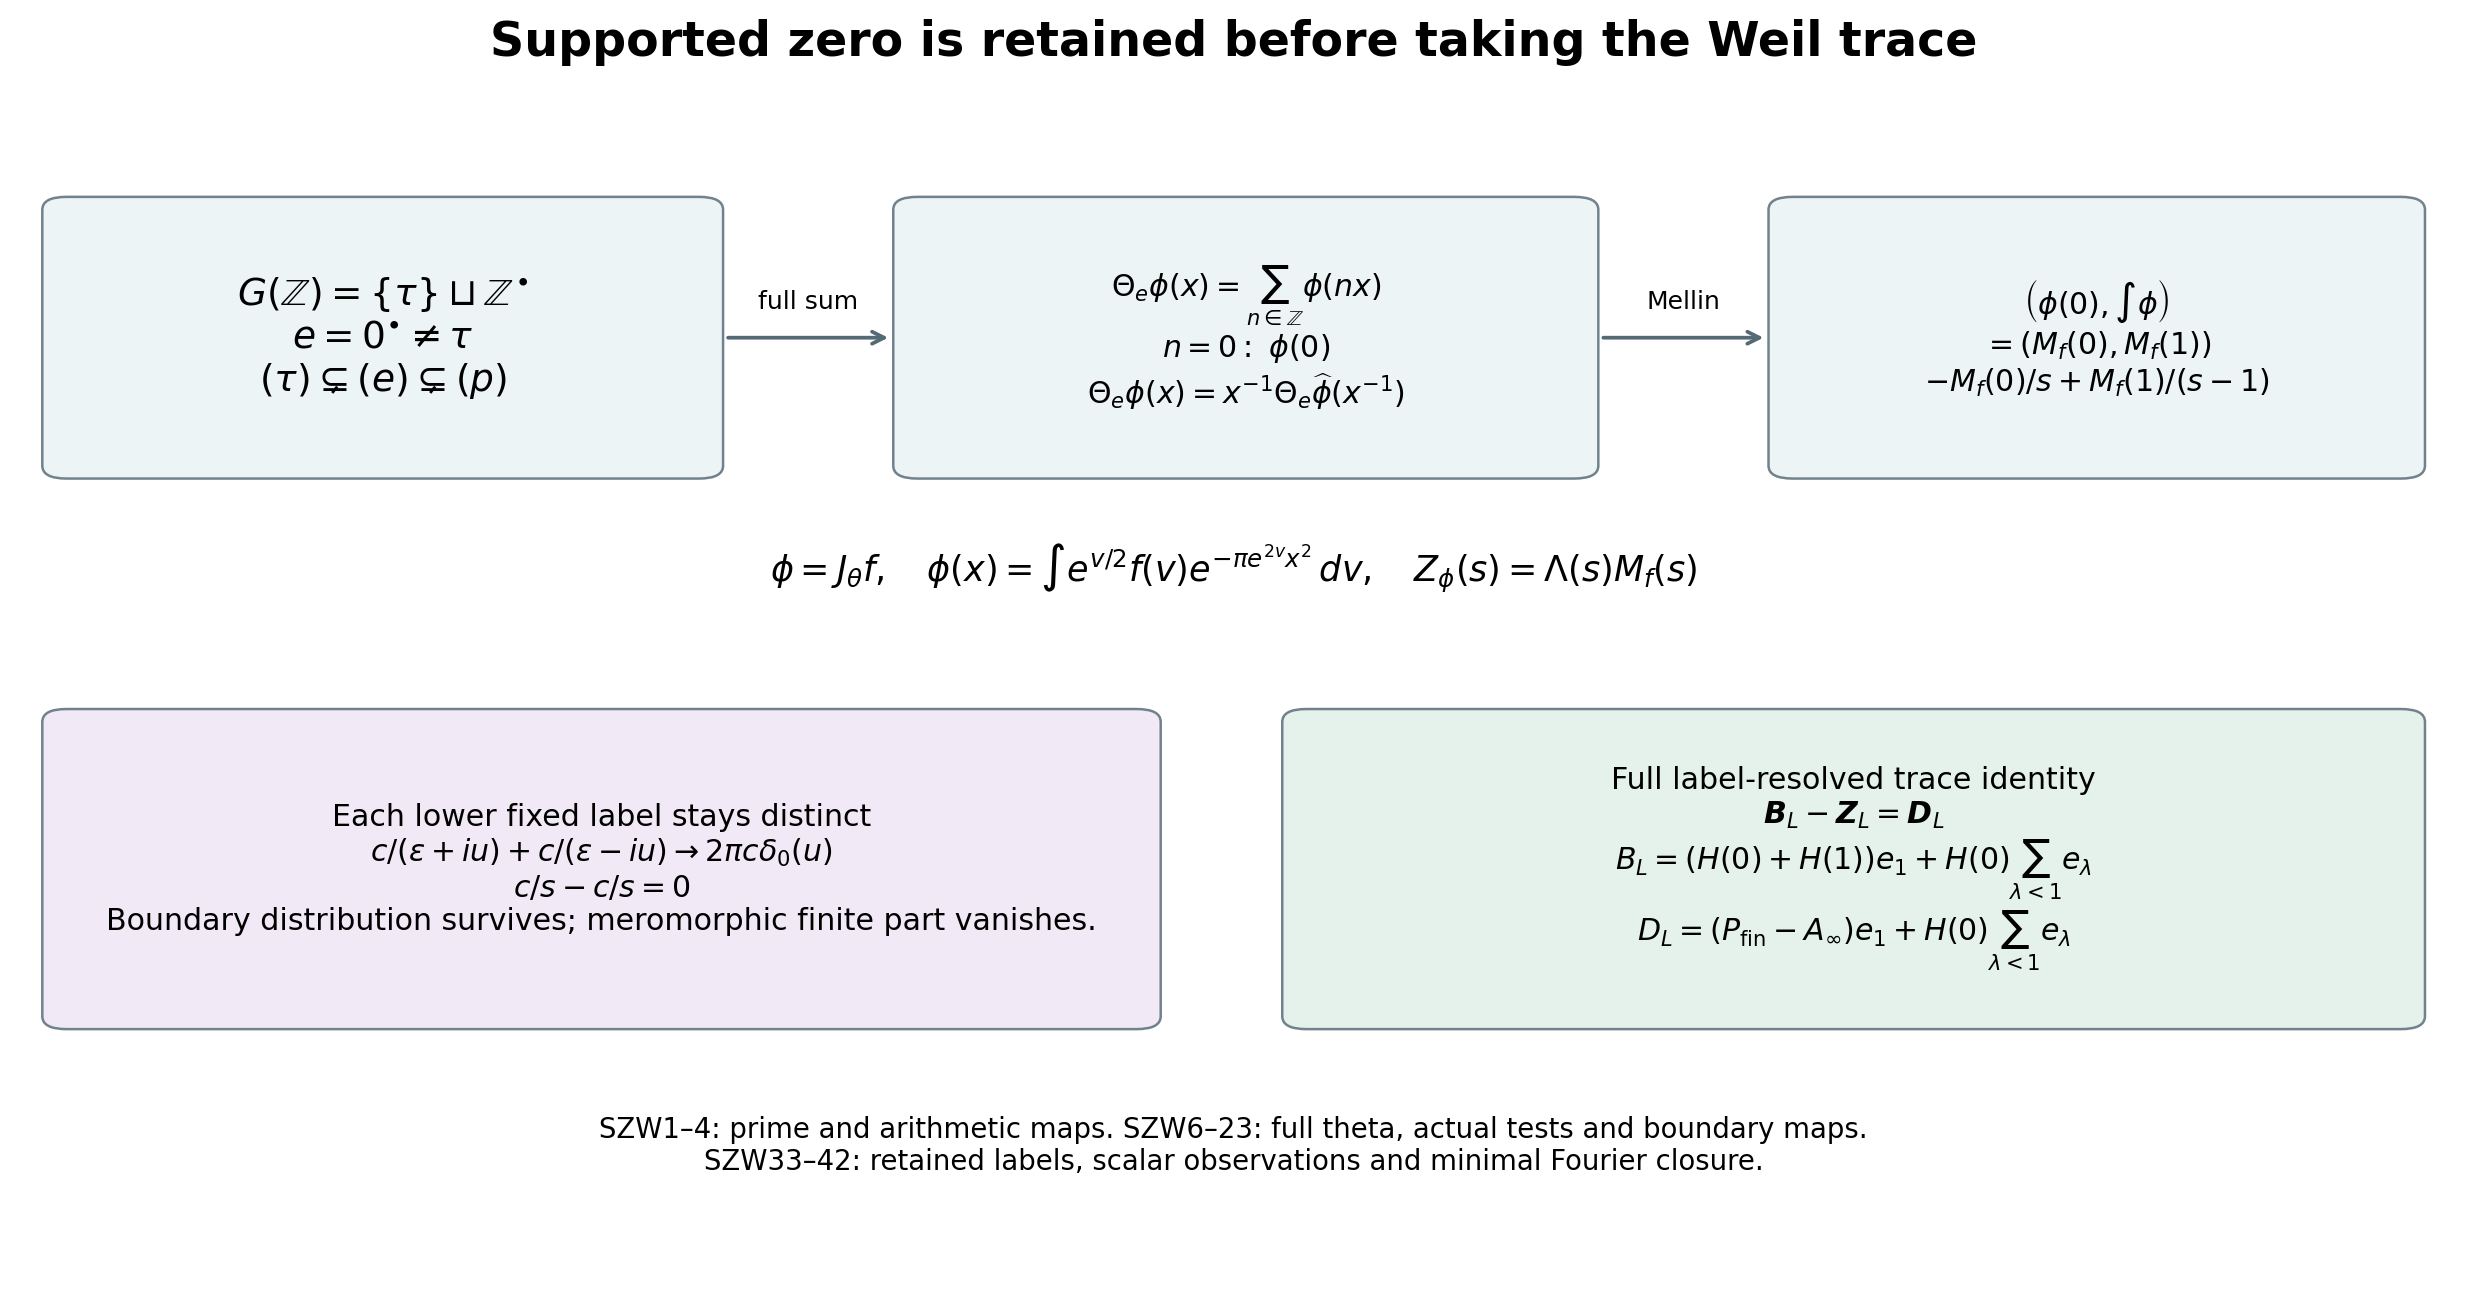
\includegraphics[keepaspectratio,alt={The actual supported-zero prime, its full theta and Mellin endpoint map, the retained fixed-support boundary distributions, and the full label-resolved trace identity. SZW1--SZW4, SZW6--SZW23 and SZW33--SZW42 prove the displayed maps and constants.}]{figures/32_supported_zero_weil.png}}
\caption{The actual supported-zero prime, its full theta and Mellin
endpoint map, the retained fixed-support boundary distributions, and the
full label-resolved trace identity. SZW1--SZW4, SZW6--SZW23 and
SZW33--SZW42 prove the displayed maps and constants.}
\end{figure}

\end{document}
